\documentclass{article}
\usepackage{natbib}
\usepackage{mathpartir}
\usepackage{stmaryrd}
\usepackage{amsthm}
\usepackage{amsmath}
\usepackage{amsfonts}
\usepackage[colorlinks=false]{hyperref}
\usepackage{graphicx}

\newcommand{\reflcompile}[1]{C(#1)}
\newcommand{\compile}[1]{\llbracket{}{#1}\rrbracket{}}
\newcommand{\dinfty}{D_{\infty}}
\newcommand{\pomega}{P_{\omega}}
\newcommand{\id}{\text{id}}
\newcommand{\projection}{\triangleleft}

\newtheorem{theorem}{Theorem}
\newtheorem{definition}{Definition}

\title{Categorical Semantics for Dynamically Typed Languages, Notes for History of Programming Languages, 2017}
\author{Max S. New, Northeastern University}
\begin{document}
\maketitle

\begin{abstract}
  These are the notes for a talk I gave for Matthias Felleisen's {\it
    History of Programming Languages} class.
  I've tried to avoid recounting detailed descriptions of category
  theory and domain theory here, which I think the cited papers
  themselves did a good job of doing.
  Instead, I've tried to take
  advantage of the connections between syntax and category theory to
  reframe some of the results in these papers as syntactic
  translations, especially the theorems in
  \ref{section:syntax:reflexive}, \ref{section:syntax:karoubi}.
\end{abstract}

\begin{section}{Historical Overview}
  In 1969, Dana Scott wrote a paper in which he said untyped lambda
  calculus had no mathematical meaning (\cite{scott1993type}), 11
  years later he wrote a paper that organized many of the different
  semantics he and others had since found using the language of
  category theory (\cite{scott80relating}). This latter paper is
  really the first deserving of the title ``categorical semantics of
  dynamic typing'', and so I'm going to present some of the theorems
  and ``theorems'' presented in that paper, but mingled with the
  history of the idea and the preceding papers that led to them.

  In \autoref{figure:timeline} we have a very skeletal timeline: On
  the left are some foundational categorical logic papers, on the
  right are some seminal semantics papers by Dana Scott that we'll go
  over in some detail throughout this article.

  I drew them in parallel, but it is clear that there was interaction
  between the sides, for instance Scott says he received a suggestion
  by Lawvere in \cite{scott1972continuous}. But what's very
  interesting is that \emph{both} Lambek and Scott wrote papers on
  cartesian closed categories and lambda calculus for the 1980 Haskell
  Curry Festschrift (\cite{lambek80lambdaccc} and
  \cite{scott80relating}), so this seems to have been something of a
  milestone for the use of category theory in programming languages.
  For completeness, since I won't discuss them in detail below, the
  Lawvere paper is \cite{lawvere1969adjointness} where Lawvere
  introduced the notion of hyperdoctrine, which allows for the
  interpretation of higher-order logic. The Lambek papers form a
  series called ``Deductive Systems and Categories I,II,III''
  (\cite{lambek68deductive}, \cite{lambek69deductive},
  \cite{lambek1972deductive}), though I confess I wasn't able to find
  copies, so I'm not quite sure which one can really be said to be the
  ``origin'' of the theorem discussed in \autoref{section:ccc}.
  \begin{figure}
    \begin{center}
      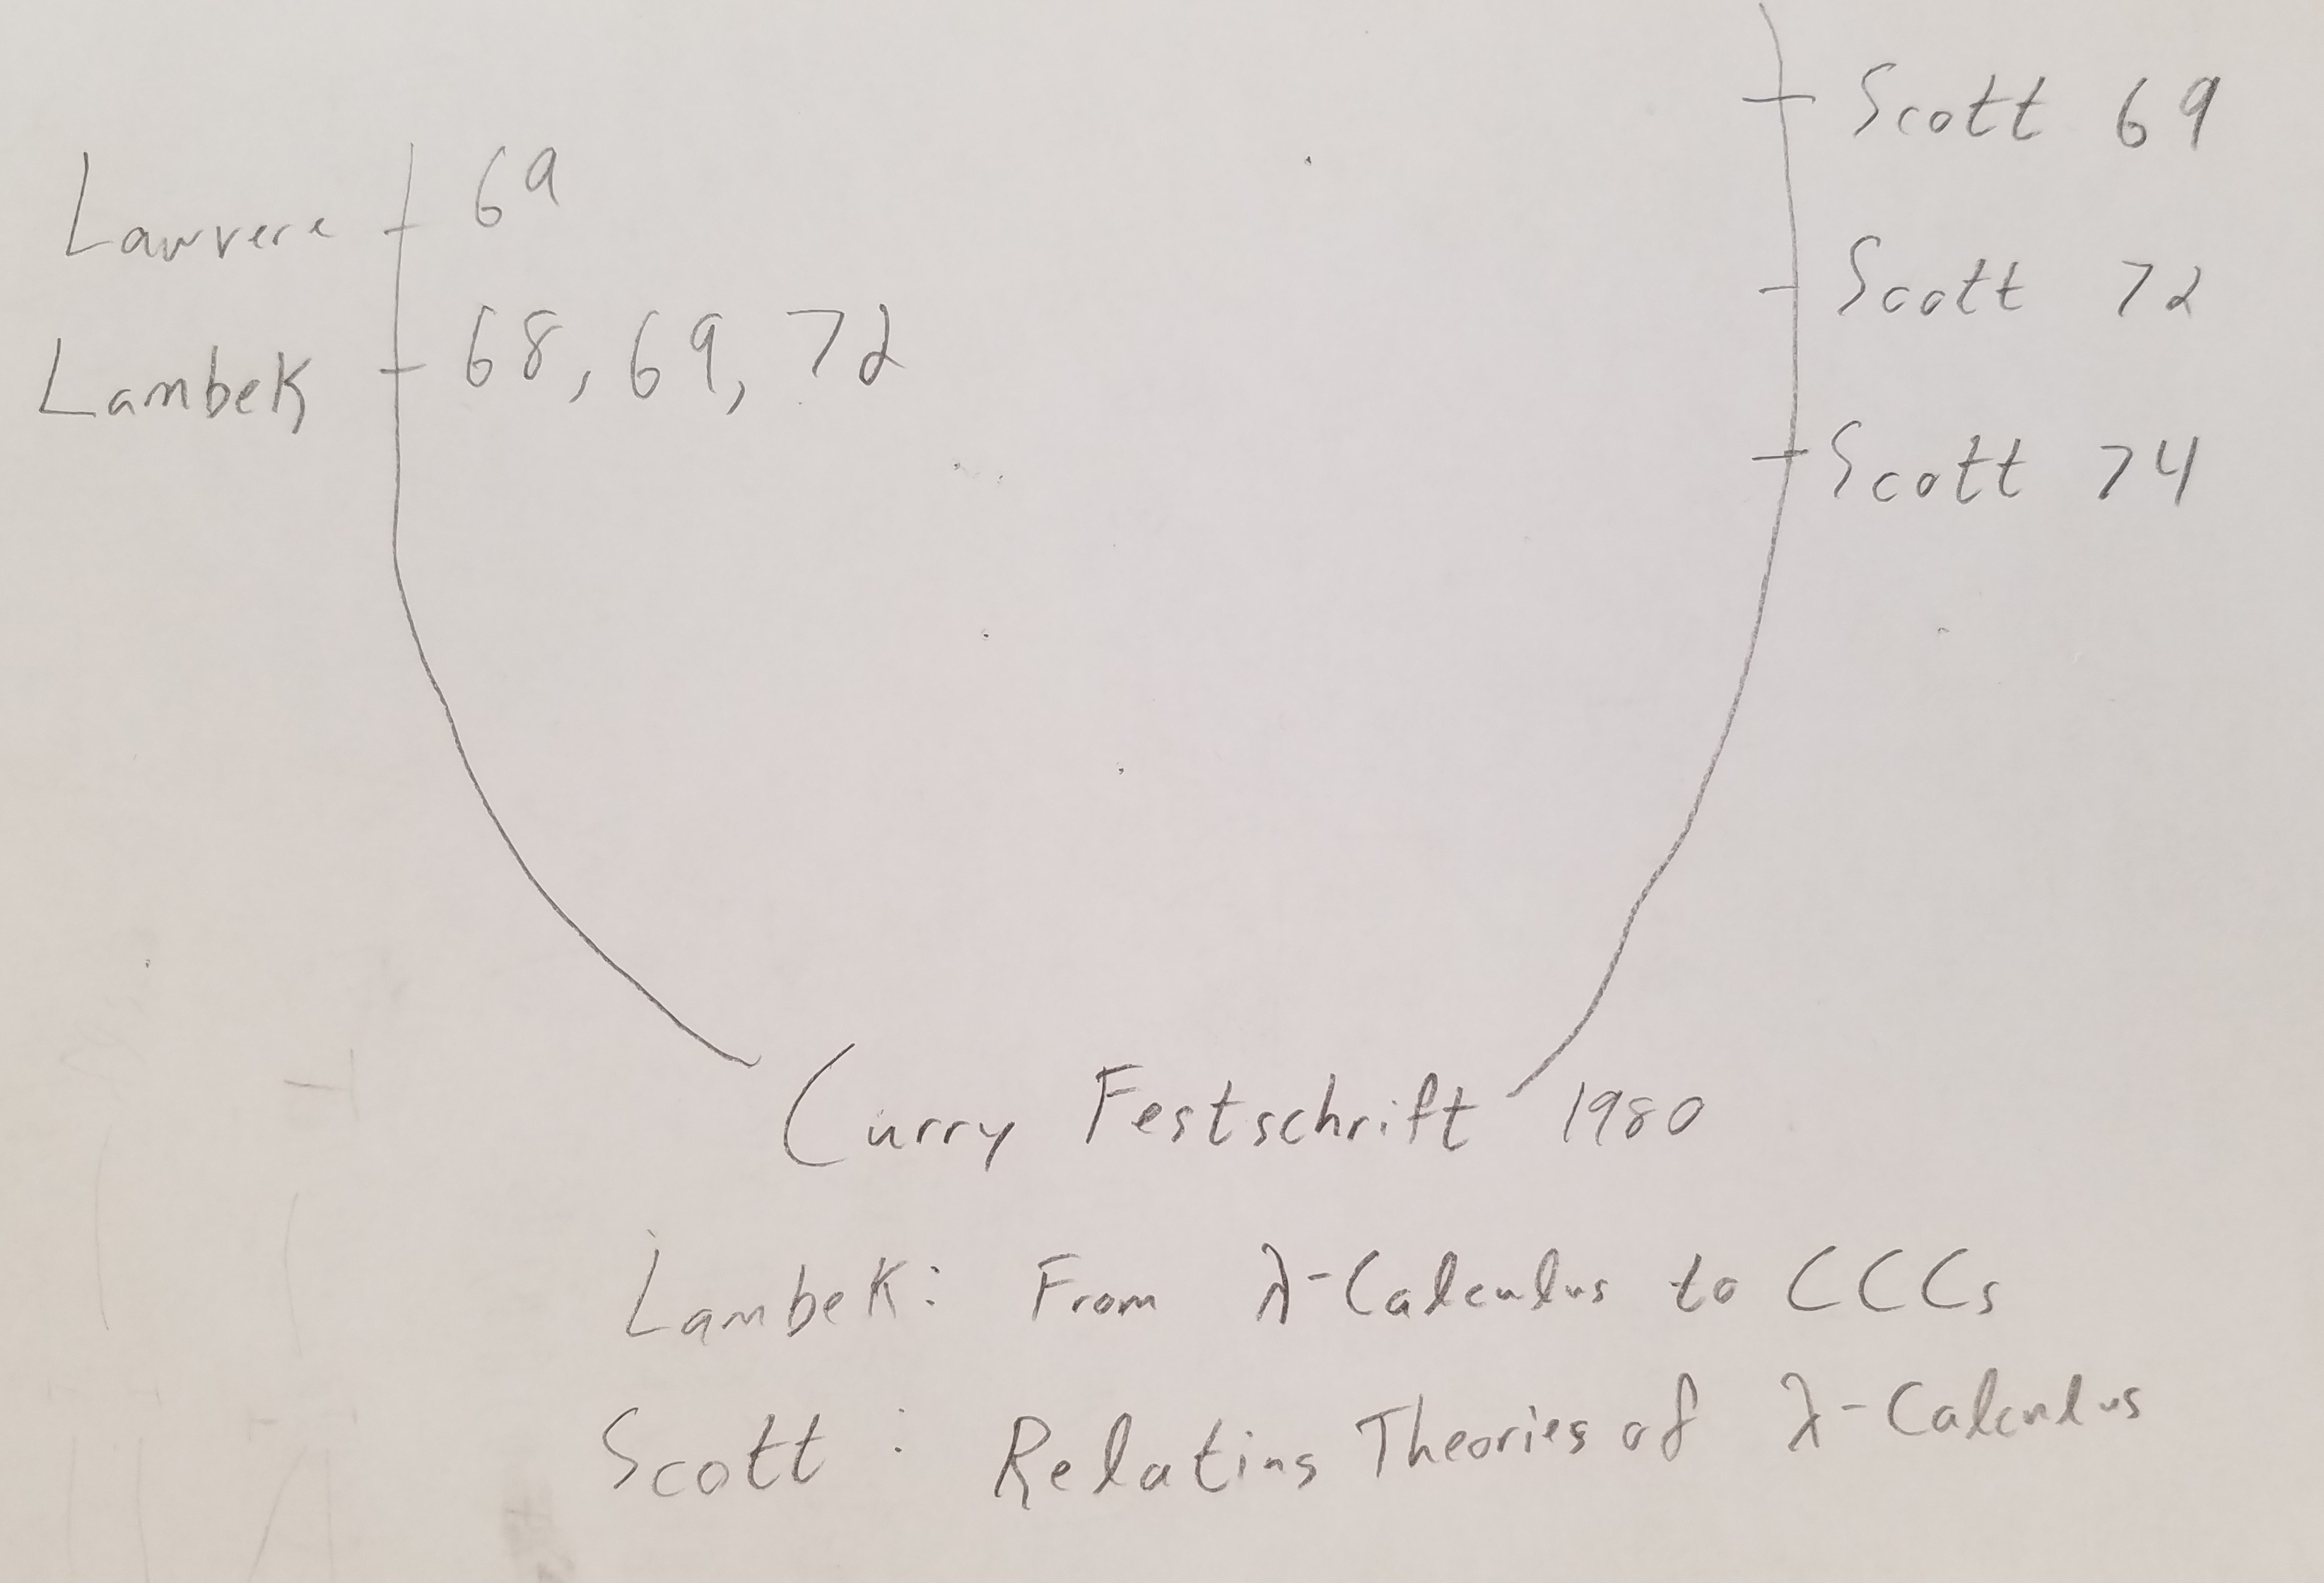
\includegraphics[height=6cm]{timeline}
    \end{center}
    \caption{Artisinally Crafted Timeline}
    \label{figure:timeline}
  \end{figure}
  % TODO: put the timeline and says something about it
\end{section}

\begin{section}{Pre-history: Scott 1969}
  % tl;dr: Scott wanted a mathematical foundation for programming
  % languages, rejected "formalist techniques" like Church-Rosser,
  % thought untyped lambda calculus could not be given a mathematical foundation

  We start in 1969, with a really remarkable unpublished manuscript by
  Dana Scott ``A type-theoretical alternative to ISWIM, CUCH, OWHY''.
  This was a very influential paper, despite never being published,
  both Mitch Wand and Matthias Felleisen confirmed to me that they had
  read it.  Basically, it lays out Dana Scott's philosophy of
  programming language semantics and already contains a fair amount of
  the foundations of domain theory.

  Dana Scott opposed the ``formalist'' approach to combinatory logic
  and programming language semantics wherein you just define a syntax
  and declare some axioms that it should satisfy without some external
  justification. He includes in this camp combinator logic (SKI) and
  the untyped lambda calculus with $\beta$ and $\eta$ laws.

  His main objection is that the axioms of said systems have no
  meaning independent of the syntax itself. He even says that we are
  lucky that these systems are consistent at all, and criticizes the
  Church-Rosser theorem, a syntactic method that proves that
  $\beta,\eta$ equality is not trivial, as a brittle approach.

  Instead he promotes a ``model-theoretic'' approach, in which you
  start with an intended mathematical semantics, and then justify your
  syntax as constructions in the model and justify your axioms by
  equations that hold in that model. In particular, the model should
  be ``independent'' from the syntax of the language itself so that
  the equalities in the models are just ``ordinary mathematics''.  In
  particular, it is desirable that the interpretation of application
  in the lambda calculus be ``real'' function application.

  Most interesting to us is that he states that he believes
  \emph{untyped} lambda calculus ``makes no sense whatsoever''.  This
  is why the paper was never published: he discovered denotational
  models of untyped lambda calculus later that very same year!

  The paper was eventually published in {\it Theoretical Computer
    Science} with historical commentary from Scott. I highly recomend
  this version to anyone that works on programing language semantics.
\end{section}

\begin{section}{Typed Lambda Calculi and Cartesian Closed Categories}
  \label{section:ccc}
  % tl;dr: be clear about what the connection is: cbn, negative typed
  % lambda
  % don't go into too much detail, there's better explanations out
  % there, but
  % describe the theorem explicitly: constructing a CCC is *the same*
  % as giving a model of λ.

  So, just as Dana Scott did, let's start with the models of
  \emph{typed lambda calculus}, also the first theorem in
  (\cite{scott80relating}).

  You've probably heard this one before: they're the cartesian closed
  categories. Now today typed lambda calculus can mean just about
  anything, so to be more precise, the theorem says that the
  call-by-name, negative, extensional typed lambda calculus
  corresponds exactly to cartesian closed categories.

  By call-by-name I mean that we have $\beta$-reduction with arbitrary
  expressions being substituted $(\lambda{x}. {t}) u = t[u/x]$ for any
  expression $u$.

  By negative, I mean that the types that correspond to structures
  present in \emph{all} cartesian closed categories are the unit type
  $1$, product type $A\times B$ and function type $A \to B$.  And by
  extensional I mean that you have $\beta$ and $\eta$ equality for all
  these connectives.

  For other flavors of lambda calculus (call-by-value, with sums and
  the empty type), you have a different theorem. But this one applied
  to the languages Dana Scott studied and was compatible with general
  recursion.

  I don't want to go into much detail because this is a very
  well-known result (see \cite{lambek1988introduction}) Without going
  into too much detail (we are supposed to talk about dynamically
  typed languages after all), here's a formulation of the
  correspondence:
  \begin{theorem}[Lambek]
    Constructing a cartesian closed category is the same as giving a
    model of the call-by-name, negative, extensional typed lambda
    calculus.
  \end{theorem}

  This theorem is very nice for the semanticist because the definition
  of cartesian closed category is easier to use than all of the syntax
  of lambda calculus.  The proof of this theorem is also not entirely
  trivial, which is why it is so useful, because contexts involve some
  amount of encoding to interpret using the cartesian structure of the
  category.

  However in this talk, we're going to use it in the opposite
  way. Since there's a correspondence, any theorem about constructing
  a cartesian closed category can be rewritten as a translation from
  lambda calculus syntax to a model. If that model itself is
  syntactic, then we just have a syntactic translation!

  % TODO? talk a bit about the history of this result.
\end{section}

\begin{section}{Untyped Lambda Calculus is modelled by Unityped Lambda Calculus}
  \label{section:syntax:reflexive}
  Ok, time for our first real construction. How do we give a model of
  untyped lambda calculus? Well, remember we want to interpret the
  calculus' application as real function application, and every term
  in the lambda calculus can be applied, so everything in untyped
  lambda calculus must be a function. On the other hand everything can
  be applied to anything so if we were to give these terms a type it
  would have to be a type $D$ so that at least we can interconvert
  between $D \to D$ and $D$. To be precise we will assume we are
  talking about some CCC with an object $D$ we will call a
  \emph{reflexive object}, that has two functions

  \[
    e : (D \to D) \to D\qquad p : D \to (D \to D)
  \]

  What relationship do these need to have in order to model untyped
  lambda calculus? Isomorphism, something weaker? Let's find out, with
  the goal of making the following theorem true:

  \begin{theorem}[Scott]
    A Cartesian Closed Category with a Reflexive Object is a model of
    Untyped Lambda Calculus.
  \end{theorem}

  By untyped lambda calculus I mean pure lambda calculus, just
  application and lambda.

  Since we are giving a model of untyped lambda calculus, that means
  to prove the theorem we need to translate untyped lambda calculus
  into typed lambda calculus with a reflexive object. So we will
  consider $e,p$ to be constants of the types given above and we will
  figure out what additional equations we need.

  Let's define the translation. The translation function will be
  called $\reflcompile{-}$.  We will compile an untyped lambda term
  $x_1,\ldots,x_n\vdash{} t$ to a typed lambda term
  $x_1:D,\ldots,x_n:D\vdash{} \reflcompile{t} : D$.

  
  \begin{mathpar}
    \begin{array}{rcl}
    \reflcompile{x} & = &x\\
    \reflcompile{\lambda x. t} & =& e(\lambda x : D. \reflcompile{t})\\
    \reflcompile{t u} &= & (p (\reflcompile{t})) \reflcompile{u}
    \end{array}
  \end{mathpar}

  To show this is a model of untyped lambda calculus, we need to show
  that we preserve equivalence of untyped lambda terms.  There are of
  course multiple choices here. The original choice is to have $\beta$
  and $\eta$, aka ``the'' lambda calculus, which I will call the
  ``untyped lambda calculus''. However, this is not so relevant to
  real dynamically typed programming languages, which have many
  different data types, these would have just $\beta$ equality for
  functions and $\eta$ will fail for those terms that are not
  functions.

  Let's start by preserving $\beta$. We need to show that

  \[ \reflcompile{(\lambda{x}. {t}) u} = \reflcompile{t[u/x]} \]

  So let's start with the left side:

  \begin{mathpar}
    \begin{array}{rcl}
      \reflcompile{{(\lambda{x}. {t}) u}} & = &  (p (e(\lambda x : D. \reflcompile{t}))) \reflcompile{u}\\
    \end{array}
  \end{mathpar}

  We'd really like to get that $\reflcompile{u}$ to be substituted
  into that lambda, so to do that we will need to add an axiom to $D$:
  that $p(e(x)) \equiv x$. The category-theoretic terminology is to
  say that $p$ is a \emph{retraction} of $e$, or that $e$ is a
  \emph{section} of $p$. Collectively, we'll call them a
  \emph{retract}.
  If $e,p$ form a retract, then we get

  \begin{mathpar}
    \begin{array}{rcl}
      \reflcompile{{(\lambda{x}. {t}) u}} & = &  (p (e(\lambda x : D. \reflcompile{t}))) \reflcompile{u}\\
      & = & (\reflcompile{t})[\reflcompile{u}/x]\\
      & = & \reflcompile{t[u/x]}
    \end{array}
  \end{mathpar}
  Where the last step follows from an easy compositionality theorem
  for our translation.

  What about $\eta$, that is $t = \lambda{x}.(t x)$? Let's calculate
  again:

  \begin{mathpar}
    \begin{array}{rcl}
      \reflcompile{{\lambda{x}.(t x)}} & = & e(\lambda{x:D}. p(\reflcompile{t})x)\\
      & = & e(p(\reflcompile{t}))
    \end{array}
  \end{mathpar}

  where the second step is the \emph{typed} $\eta$ principle (remember
  $p(\reflcompile{t}) : D \to D$). Then clearly we need $e(p(x)) =
  x$. Together with the retraction property, this would make $e,p$
  into an \emph{isomorphism}.

  We'll call an object $D$ such that $D \to D$ is isomorphic to $D$ an
  \emph{extensional} reflexive object, and when $e,p$ is just a
  section-retraction pair, we'll call it an \emph{intensional}
  reflexive object.
  Then we can refine our theorem before to pick which equations we
  want:

  \begin{theorem}
    \begin{enumerate}
    \item A CCC with an \emph{extensional} reflexive object is a model
      of untyped lambda calculus with $\beta$ and $\eta$ equality.
    \item A CCC with an \emph{intensional} reflexive object is a model
      of untyped lambda calculus with $\beta$ equality.
    \end{enumerate}
  \end{theorem}
\end{section}

\begin{section}{Constructing a Reflexive Object: $D_{\infty}$}
  Ok, so that explains how we can get untyped models from typed models
  with a reflexive object, but that doesn't tell us that there are any
  ``mathematical'' models like Scott desired.

  There's a lesson here: at its most abstract, category theory is very
  ``syntactic''. In fact in several of the earlier papers, Dana Scott
  expresses a mild disdain for category theory, but by 1980 he had
  certainly accepted it as a crucial tool for the semanticist.

  So let's get a high level view of some concrete\footnote{concrete
    has two completely opposite meanings in programming languages, to
    some syntax is concrete, to others semantics} models of untyped
  lambda calculus, the very first ones, from
  \cite{scott1972continuous}.

  At first, we seem pretty doomed by Cantor's diagonalization
  argument, how can we possibly get a set where $D \cong D \to D$?
  Just think about the cardinalities, we would have $|D| = |D|^{|D|}$,
  so the only solutions where $D$ is a set and $D \to D$ is the set of
  all functions from $D$ to $D$ are where $D = \emptyset,\{*\}$, so
  not useful as a model of lambda calculus, which we know can encode
  all natural numbers and partial computable functions on them.

  But, remember $D \to D$ is an object axiomatized by the notion of a
  cartesian closed category, there's nothing that says it has to mean
  the set of \emph{all} functions from a set $D$ to itself, and Dana
  Scott evades the paradox by considering only the \emph{continuous}
  functions.

  Now, I won't go into the full details, but suffice it to say that
  Scott defined something called \emph{continuous lattices}, which are
  sets with extra order-theoretic/topological structure that includes
  an element $\bot$ that denotes ``undefined'' or ``divergence''. Next
  he defined continuous functions on continuous lattices that
  basically ensures that if you want finite information about the
  output of a continuous function, you only need to provide finite
  information about the input, which is clearly a criterion that all
  \emph{computable} functions meet.

  Then we can ask how do we get a $D$ where $D \cong D \to D$, where
  $\to$ now means \emph{continuous} functions? Well if that holds,
  then

  \[
    D \cong (D \to D) \cong ((D \to D) \to (D \to D)) \cong \cdots
  \]

  So the idea is to build up something that looks like an infinite
  tree of $\to$s, an \emph{fixed point} of the $\to$ ``function''.
  Then we can hope to build a fixed point a la Tarski by starting with
  a continuous lattice $D_0$ and iterating:

  \begin{align*}
    D_0 & \\
    D_1 & = (D_0 \to D_0)\\
    D_2 & = (D_1\to D_1)\\
    & \vdots 
  \end{align*}
  
  In Tarski's theorem we would have $D_i \leq D_{i+1}$, and the
  equivalent we need to use is what's called an embedding-projection
  pair, which is a refinement of the idea of a section-retraction
  pair. An embedding-projection pair from $A$ to $B$ is a pair of
  $e : A \to B$ (the embedding), and $p : B \to A$ (the projection)
  such that $p\circ e = \id_{A}$ (so they form a section-retraction
  pair), and $e \circ p \leq \id_{B}$. We will refer to an
  embedding-projection pair collectively as an e-p pair and denote an
  e-p pair from $A$ to $B$ as $(e,p) : A \projection B$.

  So to construct a $D_{\infty}$, we start with any $D_0$ with a
  projection $(e_0,p_0) : D_0 \projection (D_0 \to D_0)$ (for example
  the ordered truth values work), and we start iterating, by defining:

  \begin{mathpar}
    e_{i+1} : (D_{i+1} = (D_i \to D_i)) \to (D_{i+1} \to D_{i+1})\\
    e_{i+1}(x)(y) = e_i(x(p_i(y)))\\

    p_{i+1} : (D_{i+1} \to D_{i+1})\to (D_{i+1} = (D_i \to D_i))\\
    p_{i+1}(x)(y) = p_i(y(e_i(x)))\\
  \end{mathpar}

  And then we take $\dinfty$\footnote{pronounced ``dee infinity''}
  to be the ``inverse limit'' of the projections $p$. So what does an
  element of $\dinfty$ look like?  Well it's just an infinite vector
  of elements from each $D_i$ such that they agree when you project:

  \[ \dinfty = \{ (x_i)_{i\in\mathbb{N}} | p_i(x_{i+1}) = x_{i}\} \]

  which is quite a nasty looking space, but does the job of satisfying
  $\dinfty = \dinfty \to \dinfty$.

  We can apply the same inverse limit construction to get models of
  dynamically typed languages with some booleans by instead
  constructing roughly
  $\dinfty' = \mathbb{B} \oplus (\dinfty' \to \dinfty')$ and research
  on solving these ``recursive domain equations'' went on for quite
  some time (\cite{wand1979fixed},
  \cite{smyth1982category},\cite{pitts1996relational} to name a few),
  and has even seeped into the operational world in the form of
  step-indexed logical relations (\cite{appel2001indexed},
  \cite{ahmed2004semantics}).

  So in summary, the $\dinfty$ construction is nice because it
  obviously gives a model, and we can construct many other similar
  models using the same idea.

  On the other hand, the elements we get are complicated, and the
  abundance of different constructions we got are not obviously
  comparable. How do I know that I got \emph{all} of the functions I
  want in my model?  
\end{section}

\begin{section}{Constructing a Universal Object: $P_{\omega}$}
  % Talk about the difference between Reflexive and Unversal,
  % P_{\omega},
  % advantages: constructions on types are just constructions on terms
  % (smells of contracts to me)

  So using the $\dinfty$ construction we can build many different
  models of untyped lambda, but which ones do we actually want?  If we
  want to pick a single untyped universe of values, we'd like it to
  support as many constructions as possible.

  In other words, we'd like some idea of what \emph{types} our untyped
  model can represent, and even better we'd like to get untyped models
  that represent exactly some natural classes of domains that we
  already have.

  To answer this question, we need to understand 2 things. What does
  it mean to represent a type in another? And how could we possibly
  get one of these? These ideas are all in \cite{scott1976data}.

  \begin{subsection}{Types as Retracts as Idempotents}
    When can one type represent another? Let's say I have a dynamic
    type $D$, and I'd like to be able to represent all of the
    operations of some types $X,Y,Z,\ldots$.  So for example every
    function $X\times Y \to Z$ should be implementable as a function
    $D\times D \to D$, \emph{without} exposing intensional details
    about how the function is implemented.

    Retracts work very well for this purpose. To see why, let's say we
    have retractions for $X$ and $Y$ into $D$, that is we have section
    retraction pairs $e_X : X \to D, p_X : D \to X$ with
    $p_X \circ e_X = \id_X$ and similarly $e_Y,p_Y$. Then every
    function $f : X\to Y$ can be encoded as $p_Y \circ f \circ
    e_X$. Furthermore, we can take \emph{any} function
    $\phi : D \to D$ and turn it into a function
    $e_Y \circ \phi \circ p_X : X \to Y$, and if we compose these
    processes we recover our original $f$:

    \[
      e_Y \circ (p_Y \circ f \circ e_X) \circ p_X = (e_Y \circ p_Y) \circ f \circ (e_X \circ p_X) = f
    \]

    Then we can actually \emph{identify} any $f : X \to Y$ with its
    image $p_Y \circ f \circ e_X : D \to D$, and we get the following
    natural characterization:

    \[ \text{If } \phi : D \to D, \exists f : X \to Y. p_Y\circ f
      \circ e_X = \phi \iff (e_Y \circ p_Y) \circ \phi \circ (e_X
      \circ p_X) = \phi \]

    The interesting thing to note here is that we've reduced the
    property involving multiple types to just the functions
    $(e_X\circ p_X),(e_Y\circ p_Y) : D\to D$, which we call
    $c_X,c_Y$. Since these are functions from $D$ to itself, we can
    think of them as \emph{untyped} functions. So if $X$ is a retract
    of $D$, we can describe all functions involving $X$ using $D$ and
    a single function $c_X$.

    Since $c_X$ arises from a retraction, it has a special property,
    which is that it is \emph{idempotent}: $c\circ c = c$. The
    intuition for this property comes from the section-retraction
    pairs. We think of the idempotent as a \emph{representation} of a
    retract, identifying some ``good'' subset of a dynamic type by
    coercing all elements to behave like that type. Then we can
    identify $X$ with the image of $c : D \to D$.
  \end{subsection}

  \begin{subsection}{Universal Object: $P_{\omega}$}
    So now that we've seen that retracts allow us to encode one type
    in another, we return to our goal, to construct a single type that
    characterizes some interesting class of types. This is called a
    \emph{universal type} or in category terms, a \emph{universal
      object}.

    \begin{definition}
      A category has a universal object $D$ if every object in the
      category has a section-retraction pair into $D$.
    \end{definition}

    One of the remarkable things that Dana Scott accomplished in
    \cite{scott1976data} was that he constructed a universal
    countably-based continuous lattice: $P_{\omega}$\footnote{pronounced ``pee omega''}.

    Without further ado, here it is:
    \[ \pomega = \mathbb{N} \to \{\bot, \top\} \]
    Surprised?

    The idea is that an element of $\pomega$ represents a subset of
    the natural numbers, and an element of a countably-based
    continuous lattice is determined by all of the observations you
    can make on it. So if you have a lattice $X$ with countable basis
    $b_i$, then you can define the embedding as

    \begin{mathpar}
      e : X \to \pomega\\
      e(x) = \{ i | b_i \sqsubseteq x \}
    \end{mathpar}
    Where $b_i \sqsubseteq x$ essentially means that some finite
    observation $b_i$ holds of $x$.

    The projection, on the other hand, is less nice:

    \begin{mathpar}
      p : \pomega \to X\\
      p(S) = \bigsqcup\{ b_i | i \in S \}
    \end{mathpar}

    Where that $\bigsqcup$ corresponds operationally to a parallel
    exists, which is an impractical feature to have in your
    programming language (\cite{plotkin1977lcf}).

    While this universal type may be infeasible for a programming
    language implementation, the semantic properties it has are quite
    enticing!  First, since every type is a retract of $\pomega$, we
    can understand all continuous functions by studying
    $\pomega \to \pomega$. More concretely, since retracts are
    determined by their idempotents, we can study constructions on
    \emph{types} by functions on \emph{terms}.

    For example, instead of constructing non-well-founded recursive
    types by methods like $\dinfty$, you can just use ordinary
    recursion on terms, much simpler!

    Finally, while we can't use $\pomega$ in our sequential languages,
    it turns out that many languages do have universal types. For a
    more thorough overview and much better exposition than here, I
    highly recommend \cite{Longley2003}.
  \end{subsection}
\end{section}

\begin{section}{Translating Typed to Untyped: All Untyped Models are Unityped Models}
  \label{section:syntax:karoubi}

  Based on last section, we can turn the idea around, instead of
  taking our typed model and looking for an untyped model that
  ``generates it'', we might just start with our untyped language and
  see what ``types'' we can get from it.

  This idea gets us to the main theorem of \cite{scott80relating}:
  \begin{theorem}
    Any model of untyped lambda calculus is embedded as a reflexive
    object in a cartesian closed category.
  \end{theorem}
  That is, from a model of untyped lambda calculus, we can
  \emph{construct} a cartesian closed category with a reflexive object
  such that the functions in the untyped model are exactly the
  endo-functions of the reflexive object.

  Remembering the correspondence between typed lambda calculus and
  cartesian closed categories, \emph{constructing} a CCC is the same
  as defining a \emph{translation} of the typed lambda calculus, so
  the proof of this theorem is actually a translation from typed to
  untyped lambda calculus.

  The intuition for the translation comes from the previous section:
  we want the types to be retracts of the dynamic type, so we will
  interpret the types as exactly the idempotent they represent on the
  dynamic type, which is then just an untyped lambda term!

  So first, we interpret the types of the lambda calculus as untyped
  terms $c$ such that $c(c x) \equiv c x$.

  \begin{mathpar}
    \begin{array}{rcl}
      \compile{1} & = & \lambda x.()\\
      \compile{A\times B} & = & \lambda p. (\compile{A}(\pi_1 p), \compile{B}(\pi_2 p))\\
      \compile{A\to B} & = & \lambda f. \lambda x. \compile{B}(f(\compile{A} x))
    \end{array}
  \end{mathpar}

  Which you may recognize as (except the $1$) case, basically the
  corresponding contracts from \cite{findler2002contracts}. I'll leave
  it as an exercise that these are actually idempotent.

  Next, we want to translate typed terms to untyped terms, but in such
  a way that we maintain the validity of $\beta,\eta$ equivalence. How
  can we achieve this? When you expand the domain of a function, you
  can call it on new inputs, so we have to make sure that these new
  inputs don't reveal any new information about our terms. That is,
  the equality for the untyped translation of a typed term should be
  completely determined by its behavior linking with other typed
  terms.

  Fortunately, the interpretation of types above coerces \emph{any}
  untyped term to behave like a term of a given type. So we just need
  to make sure that any interaction with a dynamically typed term is
  mediated by one of these idempotents.

  It turns out that it's very simple to
  derive a translation that validates this equation, we just need to
  put idempotents on the variables!

  \begin{mathpar}
    \begin{array}{rcl}
      \compile{x : A} & = & \compile{A} x\\
      \compile{\lambda (x:A). t}  & = & \lambda x. \compile{t}\\
      \compile{t u}  & = & \compile{t}\compile{u}\\
      \compile{(t,u)}  & = & (\compile{t},\compile{u})\\
      \compile{\pi_i t}  & = & \pi_i \compile{t}\\
      \compile{()} & = & ()
    \end{array}
  \end{mathpar}

  In order to prove preservation of $\eta$, we prove the following
  soundness theorem.

  \begin{theorem}[Soundness]
    \label{theorem:soundness}
    {~}\\
    If $x_1:A_1,\ldots,x_n:A_n\vdash{} t : B$, then
    $x_1,\ldots,x_n\vdash{} \compile{t}$ and
    \[
      \compile{B}(\compile{t}[(\compile{A_1} x_1)/x_1\cdots]) \equiv_{\beta} \compile{t}
    \]

    equivalently,

    \[
      \compile{B}(\compile{t}) \equiv_{\beta} \compile{t} \equiv_{\beta} \compile{t}[(\compile{A_1} x_1)/x_1\cdots]
    \]
    
  \end{theorem}

  Clearly the second formulation implies the first. To see the other
  direction, if we have $\compile{B}(\compile{t})$, then

  \begin{mathpar}
    \begin{array}{rcl}
      \compile{B}(\compile{t}) & \equiv_{\beta} & \compile{B}(\compile{B}(\compile{t}[(\compile{A_1} x_1)/x_1\cdots]))\\
      & \equiv_{\beta} & \compile{B}(\compile{t}[(\compile{A_1} x_1)/x_1\cdots])\\
      & \equiv_{\beta} & \compile{t}
    \end{array}
  \end{mathpar}
  Where the second equation is from $\compile{B}$ being idempotent.

  What does this have to do with validating $\eta$? Well if we look at
  the definitions of the $\compile{A}$s, we see that they are
  performing $\eta$ expansion!

  \begin{theorem}[Soundness implies Eta Preservation]
    If $\autoref{theorem:soundness}$ is true, then
    \begin{enumerate}
    \item If $t : A \to B$, then $\lambda x. \compile{t} ({\compile{A}x}) \equiv_{\beta} \compile{t}$.
    \item If $t : A \times B$, then $(\pi_1 \compile{t},\pi_2 \compile{t}) \equiv_{\beta} \compile{t}$.
    \item If $t : 1$, then $() \equiv_{\beta} \compile{t}$.
    \end{enumerate}
  \end{theorem}
  \begin{proof}
    We'll do the first case, the others are similar.  By soundness,
    $\compile{A\to B}(\compile{t}) \equiv_{\beta} \compile{t}$, expanding
    the definition this means:
    \begin{mathpar}
      \begin{array}{rcl}
        \lambda x. \compile{t} ({\compile{A}x})
        & \equiv_{\beta} & \lambda x. (\compile{A\to B}\compile{t}) ({\compile{A}x})\\
        & \equiv_{\beta} & \lambda x. (\lambda y. \compile{B}(\compile{t} ({\compile{A}y})))(\compile{A} x)\\
        & \equiv_{\beta} & \lambda x. \compile{B}(\compile{t} ({\compile{A}(\compile{A} x)}))\\
        & \equiv_{\beta} & \lambda x. \compile{B}(\compile{t} (\compile{A} x))\\
        & \equiv_{\beta} & \compile{A\to B}\compile{t}\\
        & \equiv_{\beta} & \compile{t}\\
      \end{array}
    \end{mathpar}
    where the fourth equality is from idempotence of $\compile{A}$.
  \end{proof}

  So this shows that $t$ is compiled in such a way that all
  interactions are protected by the idempotents
  $\compile{A_i},\compile{B}$. 

  So it remains to prove the soundness theorem
  \begin{proof}
    By induction on $t$. We do a few illustrative cases
    \begin{enumerate}
    \item $t = x : A$, then
      \begin{mathpar}
        \begin{array}{rcl}
          (\compile{A}(\compile{A}x))[(\compile{A}x)/x] & = & \compile{A}(\compile{A}(\compile{A} x))\\
                                                        & = & \compile{A}(\compile{A} x)\\
                                                        & = & (\compile{A} x)\\
        \end{array}
      \end{mathpar}
    \item $t = \lambda (x:A). u$, then
      \begin{mathpar}
        \begin{array}{rcl}
          \compile{A\to B}(\lambda x. \compile{u})[\cdots] & = & \lambda y. \compile{B}((\lambda x. \compile{u}[\cdots]) (\compile{A} y))\\
          & = & \lambda y. \compile{B}\compile{u}[(\compile{A} y)/x,\cdots]\\
          & = & \lambda y. \compile{u}[y/x]\\
          & = & \compile{\lambda(x:A).u}\\
        \end{array}
      \end{mathpar}
    \item $t = t' u$, then
      \begin{mathpar}
        \begin{array}{rcl}
          \compile{B}(\compile{t'} \compile{u})[\cdots]
          & = & \compile{B}(\compile{t'}[\cdots] \compile{u}[\cdots])\\
          & = & \compile{B}(\compile{t'} \compile{u})\\
          & = & \compile{B}((\compile{A\to B}\compile{t'}) \compile{u})\\
          & = & \compile{B}((\lambda x. \compile{B}(\compile{t'} (\compile{A} x))) \compile{u})\\
          & = & \compile{B}(\compile{B}(\compile{t'} (\compile{A} \compile{u})))\\
          & = & \compile{B}(\compile{t'} (\compile{A} \compile{u}))\\
          & = & (\lambda x. \compile{B}(\compile{t'} (\compile{A} x)))\compile{u}\\
          & = & (\compile{A\to B}\compile{t'})\compile{u}\\
          & = & \compile{t'}\compile{u}\\
        \end{array}
      \end{mathpar}
    \end{enumerate}
  \end{proof}

  
\end{section}

\begin{section}{Looking Forward}
  What can we glean today from Dana Scott's semantic insights?

  Personally, I'm interested in gradual typing and I've found the
  ideas in \cite{scott80relating} very illuminating in this regard.
  The hope is that by taking a bit more abstract of a perspective, we
  can prove some general results for constructing gradually typed
  languages.  For example, the category constructed in
  \autoref{section:syntax:karoubi} is called the ``Cauchy completion''
  or ``Karoubi envelope'' and this abstract perspective can be used to
  show that the construction of idempotents always works to validate
  $\eta$ laws. Susumu Hayashi has an interesting paper about this idea
  \cite{hayashi1985adjunction}, and I think it goes a long way to
  explaining why gradual typing has extended to so many language
  features.
\end{section}

\newpage
\bibliographystyle{plainnat}
\bibliography{dyn-cats}

\end{document}
